\section{Calculating $e$}

\epigraphwidth=0.75\textwidth
\epigraph{\emph{Let us change our traditional attitude to the
    construction of programs. Instead of imagining that our main task is
    to instruct a computer what to do, let us concentrate rather on
    explaining to human beings what we want a computer to do.}}
    {---Donald Knuth}

\noindent
The number $e$, also known as \emph{Euler's number} (Leonhard Euler,
1707--1783), is an irrational mathematical constant approximately
equal to $2.71828$, that appears pervasively in the natural and
mathematical worlds. It is the base of the natural logarithm, it
is the limit of $\lim_{n\rightarrow\infty} (1 + \frac{1}{n})^n$
which was discovered by Jacob Bernoulli in his work on the calculation
of compound interest. And, of course, it can be expressed as the
Taylor series: $$ e=\sum_{k=0}^\infty \frac{1}{k!} =
1+\frac{1}{1}+\frac{1}{2}+\frac{1}{6}+\frac{1}{24}+\frac{1}{120}+\frac{1}{720}+\frac{1}
{5040}+\frac{1}{40320}+\frac{1}{362880}+\frac{1}{3628800}+\cdots
$$

How many terms must you compute? Fewer than you might expect, since $k!$
grows very fast. You will be determining that experimentally as part of this assignment.

\begin{figure}[bth]
\begin{centering}
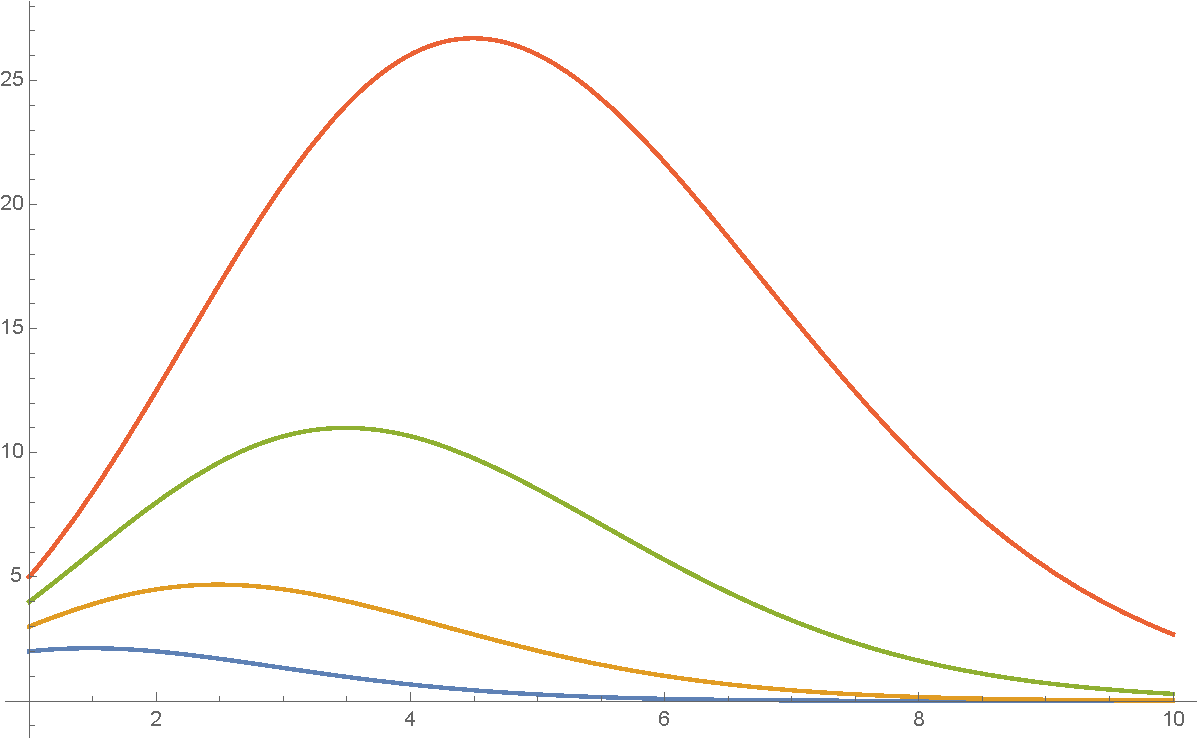
\includegraphics[width=0.75\textwidth]{images/growth.pdf}
\caption{Comparing $\dfrac{x^k}{k!}$ for $x=2,3,4,5$.}\label{growth}
\end{centering}
\end{figure}

If we are na\"ive about computing the terms of the series we can quickly
get into trouble --- the values of $k!$ get large \emph{very quickly}.
We can do better if we observe that:
$$
\frac{x^k}{k!} = \frac{x^{k-1}}{(k-1)!} \times \frac{x}{k} .
$$

At first, that looks like a recursive definition (and in fact, you could
write it that way, but it would be wasteful). As we progress through the
computation, assume that we know the previous result. We then just have
to compute the next term and multiply it by the previous term. At each
step we just need to compute $\frac{x}{k}$, starting with $k = 0!$
(remember $0! = 1$) and multiply it by the previous value and add it
into the total. It turns into a simple \texttt{for} or \texttt{while}
loop.
